% 2007 年湖南卷理科第 19 题：山坡面与水平面 α 成角 θ（sinθ=2/5），P 在坡上，
%   PH⊥α 于 H，PB⊥AB 于 B，OA⊥AB 于 A，AB 为山脚公路，D、E 在 AB 上。
% 来源 PDF：gaokaomath-src/普通高考/2007/2007湖南理.pdf
% SHA-256：80aed7d118362bf1e1ad84e6fdbb7d2a10d0ca0d3148e2cbb9e934bba996e352
% 原页：2007湖南理.pdf 第 2 页（A3 三栏）第 1 栏，书页码 380。
% 重绘依据：原页为山坡照片加线条，本库按题设几何关系重绘为示意图：
%   α 画成平行四边形，AB 为山脚线；山坡面画成 A-B-B'-A' 的平行四边形，
%   P 取在过 B 的坡面母线上，H 为 P 在 α 内的射影，PH 画虚线。
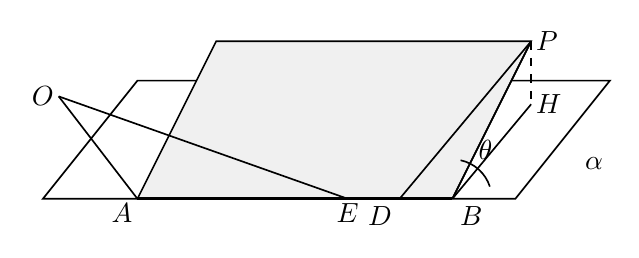
\begin{tikzpicture}[semithick, every node/.style={inner sep=1.5pt}]

  % 水平面 α
  \draw (0,0) -- (6,0) -- (7.2,1.5) -- (1.2,1.5) -- cycle;
  \node at (7.0,0.45) {$\alpha$};

  % 山坡面
  \coordinate (A) at (1.2,0);
  \coordinate (B) at (5.2,0);
  \coordinate (A2) at (2.2,2.0);
  \coordinate (B2) at (6.2,2.0);
  \fill[gray!12] (A) -- (B) -- (B2) -- (A2) -- cycle;
  \draw (A) -- (A2) -- (B2) -- (B);

  % 山脚公路 AB
  \draw[line width=1.1pt] (A) -- (B);

  % P、H、O
  \coordinate (P) at (6.2,2.0);
  \coordinate (H) at (6.2,1.2);
  \coordinate (O) at (0.2,1.3);
  \draw[dashed] (P) -- (H);
  \draw (H) -- (B);
  \draw (B) -- (P);
  \draw (O) -- (A);

  % D、E 及折线
  \coordinate (D) at (4.53,0);
  \coordinate (E) at (3.87,0);
  \draw (P) -- (D);
  \draw (E) -- (O);

  % 角 θ（BH 与 BP 之间）
  \draw (5.2,0) ++(18:0.5) arc[start angle=18, end angle=78, radius=0.5];
  \node at (5.62,0.62) {$\theta$};

  \node[left] at (O) {$O$};
  \node[below left] at (A) {$A$};
  \node[below right=1pt] at (B) {$B$};
  \node[below left=1pt] at (D) {$D$};
  \node[below] at (E) {$E$};
  \node[right] at (P) {$P$};
  \node[right] at (H) {$H$};
\end{tikzpicture}
